\documentclass[aspectratio=1610]{beamer}
\usetheme[we]{uantwerpen}
\usepackage[english]{babel}

\usepackage{metalogo}
\usepackage{kantlipsum}
% \usepackage{pgfplots}
\usepackage{booktabs}

\newcommand*\command[1]{{\tt \textbackslash #1}}
\NewEnviron{codesnippet}[1][0.8\textwidth]{
  \scriptsize
  \qquad\framebox[#1][l]{\texttt{
      \setlength\textwidth{#1}
      \begin{minipage}{0.9\textwidth}
        \BODY
      \end{minipage}
    }
  }
}
\newcommand*\ind[1][2ex]{\hspace*{#1}}
\newcommand*\bframe[1][]{\command{begin}\{#1frame\}}
\newcommand*\eframe[1][]{\command{end}\{#1frame\}}

\usepackage{graphicx}
\usepackage{caption}
% \captionsetup[figure]{labelformat=empty, justification=centering}

\usepackage{dirtytalk}
\usepackage{makecell}
\usepackage{mathtools}
\usepackage{amssymb}


\title{Matrix Factorization}
\subtitle{Collaborative Filtering for Implicit Feedback Datasets}
\date{21/12/2021}
\author{Andrei Bondarenko \& Geert Goemaere}


\begin{document}

\begin{frame}[negativefill]
  \maketitle
\end{frame}

\begin{frame}
    {Content}
\end{frame}

\begin{frame}{Collaborative Filtering for implicit feedback datasets}
\begin{itemize}
    \item Recommenders moved from explicit (ratings) to implicit (behaviour) feedback
    \item Implicit feedback characteristics
        \begin{itemize}
            \item Negative feedback not in observed information
            \item Implicit data is dense: Negative feedback in \textit{missing interactions}
            \item Feedback expressed as confidence that an item is preferred 
            \item Focus on ranking instead of rating prediction 
        \end{itemize}
    \end{itemize}
\end{frame}

\begin{frame}{Model}{Preference}
    User-item observations $r_{ui}$
    \begin{equation*}
        r_{ui} \begin{dcases*}
            > 0 & number of user-item observations \\
            = 0 & no user-item observations
            \end{dcases*}
    \end{equation*}
    
    Preference $p_{ui}$ of user \textit{u} for item \textit{i}
    \begin{equation*}
        p_{ui} = \begin{dcases*}
            1 & $r_{ui} > 0$ \\
            0 & $r_{ui} = 0$
            \end{dcases*}
    \end{equation*}
\end{frame}

\begin{frame}{Model}{Confidence}
    \begin{equation*}
        c_{ui} = 1 + \alpha r_{ui}
    \end{equation*}
    \begin{itemize}
        \item $c_{ui}$ measures confidence in observing $p_{ui}$
        \begin{itemize}
            \item the more observations $p_{ui}$, the higher the confidence
            \item minimal confidence for unobserved items (negative feedback)
        \end{itemize}
        \item $\alpha$ is \textit{rate of increase}
    \end{itemize}
\end{frame}

\begin{frame}{Goal}
    Find
    \begin{itemize}
        \item Vector $x_u \in \mathbb{R}^f$ for each user
        \item Vector $y_i \in \mathbb{R}^f$ for each item
    \end{itemize}
    Such that
    \begin{itemize}
        \item $p_{ui} = x_{u}^{T} y_{i}$
    \end{itemize}
    Difference with matrix factorization for explicit feedback
    \begin{itemize}
        \item account for varying confidence levels
        \item optimization accounts for all user-item pairs
        \begin{minipage}[b][\textheight][t]{0.59\linewidth}
        \begin{itemize}
            \item Can no longer use SGD
            \item Use ALS for optimization
        \end{itemize}
        \end{minipage}
        \begin{minipage}[b][\textheight][t]{0.39\linewidth}
        \centering
        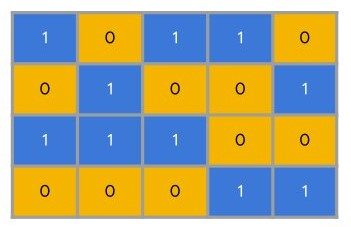
\includegraphics[trim={0 2cm 0 0},clip,width=\textwidth]{img/UnobservedEntries.jpg}
        \end{minipage}
    \end{itemize}

\end{frame}

\begin{frame}{Cost function}
    \begin{equation}
        \min_{x_{*}, y_{*}} = \sum_{u,i} c_{ui}\left( p_{ui} - x_{u}^{T} y_{i} \right)^2 + \lambda \left( \sum_{u} \left\Vert x_u \right\Vert^2 + \sum_{i} \left\Vert y_i \right\Vert^2 \right)
    \end{equation}
    \begin{itemize}
        \item Cost function contains $m \cdot n$ terms (m users, n items)
        \item Prevents use of SGD
        \item alternating-least-squares (ALS)
        \begin{itemize}
            \item compute user-factors and keep item-factors fixed
            \item compute item-factors and keep user-factors fixed
            \item repeat until convergence
        \end{itemize}
    \end{itemize}
\end{frame}

\begin{frame}{Overcoming dense cost function}
Differentiation of loss function, fixing item factors
\begin{equation}
    x_u = \left(Y^T C^u Y + \lambda \mathbb{I})\right)^{-1} Y^T C^u p(u)
\end{equation}
\begin{itemize}
    \item $C^u$ is nxn matrix where $C_{ii}^u = c_{ui}$
    \item $p(u) \in \mathbb(R)^n$ contains all preference values $p_{ui}$
    \item $Y^T C^u Y$ is $\mathcal{O}(f^2n)$ for each of $m$ users
    \item Speed up: $Y^T C^u Y = Y^TY + Y^T\left(C^u - \mathbb{I}
    \right)Y$
    \item pre-compute $Y^TY$ (independent of u)
    \item $C^u - \mathbb{I}$ has $n_u$ non-zero elements with $n_u \ll n$
    \item $C^u p(u)$ has $n_u$ elements
    \item $\mathcal{O}(f^2\mathbb{N} + f^3m)$ for all users with $\mathbb{N} = \sum_{u}n_u$
    \item Run-time scales linearly with size of data
\end{itemize}
Similar computation for
\begin{equation}
    y_i = \left(X^TC^iX + \lambda \mathbb{I})\right)^{-1} X^T C^i p(i)
\end{equation}
\end{frame}

\begin{frame}{Conclusions}
\end{frame}

\end{document}